\documentclass[aspectratio=169]{beamer}
\usetheme{Madrid}
\usecolortheme{seahorse}

\usepackage{graphicx}
\usepackage{booktabs}
\usepackage{tikz}
\usepackage{listings}
\usepackage{xcolor}

\definecolor{pardotblue}{RGB}{41,98,255}
\definecolor{pardotgray}{RGB}{60,60,60}
\definecolor{codegreen}{RGB}{0,128,0}
\definecolor{codegray}{RGB}{128,128,128}

\setbeamercolor{title}{fg=white,bg=pardotblue}
\setbeamercolor{frametitle}{fg=white,bg=pardotblue}
\setbeamercolor{structure}{fg=pardotblue}
\setbeamercolor{block title}{bg=pardotblue,fg=white}

\lstset{
  basicstyle=\ttfamily\scriptsize,
  keywordstyle=\color{pardotblue}\bfseries,
  commentstyle=\color{codegreen},
  stringstyle=\color{codegray},
  breaklines=true,
  frame=single,
  backgroundcolor=\color{gray!5},
}

\title{Pardot: AI Teaching Assistant for CS Education}
\subtitle{Scaling Personalized Support Without Scaling Staff}
\author{CS Department}
\date{\today}

\begin{document}

% --- Slide 1: Title ---
\begin{frame}
\titlepage
\end{frame}

% --- Slide 2: Problem ---
\begin{frame}{The Problem: Faculty Are Stretched Thin}
\begin{columns}[T]
\begin{column}{0.5\textwidth}
\textbf{Grading}
\begin{itemize}
  \item 200+ students per section
  \item 8--12 hours per assignment cycle
  \item Inconsistent feedback across TAs
  \item Delayed turnaround hurts learning
\end{itemize}
\end{column}
\begin{column}{0.5\textwidth}
\textbf{Student Support}
\begin{itemize}
  \item Questions at all hours (especially before deadlines)
  \item Repetitive clarification requests
  \item Office hours don't scale
  \item Students hesitate to ask ``dumb questions''
\end{itemize}
\end{column}
\end{columns}
\vfill
\begin{center}
\textit{Result: Faculty burnout, students underserved.}
\end{center}
\end{frame}

% --- Slide 3: Solution ---
\begin{frame}{The Solution: Pardot --- AI TA in Your Workflow}
\begin{block}{What is Pardot?}
An AI teaching assistant that integrates directly into the tools students and faculty already use.
\end{block}
\vspace{0.5em}
\begin{itemize}
  \item \textbf{Always available} --- 24/7 support in Discord
  \item \textbf{Course-aware} --- trained on your syllabus, assignments, and rubrics
  \item \textbf{Pedagogically sound} --- scaffolds learning instead of giving answers
  \item \textbf{Grading support} --- consistent, rubric-aligned feedback at scale
  \item \textbf{Faculty control} --- instructors set boundaries and review outputs
\end{itemize}
\end{frame}

% --- Slide 4: Setup ---
\begin{frame}{Setup: Three Integrations, One TA}
\begin{columns}[T]
\begin{column}{0.33\textwidth}
\begin{center}
\textbf{Discord}\\[0.5em]
\small
Students ask questions in course channels.
Pardot responds with scaffolded guidance.
\end{center}
\end{column}
\begin{column}{0.33\textwidth}
\begin{center}
\textbf{GitHub}\\[0.5em]
\small
Monitors repositories for submissions.
Runs automated code review and grading.
\end{center}
\end{column}
\begin{column}{0.33\textwidth}
\begin{center}
\textbf{Course Materials}\\[0.5em]
\small
Ingests syllabi, lecture notes, rubrics, and past exams for context.
\end{center}
\end{column}
\end{columns}
\vfill
\begin{center}
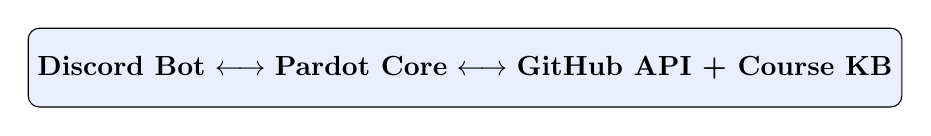
\begin{tikzpicture}
\node[draw, rounded corners, fill=pardotblue!10, minimum width=10cm, minimum height=1cm] {
  \textbf{Discord Bot} $\longleftrightarrow$ \textbf{Pardot Core} $\longleftrightarrow$ \textbf{GitHub API + Course KB}
};
\end{tikzpicture}
\end{center}
\end{frame}

% --- Slide 5: Student Interaction Example 1 ---
\begin{frame}{Student Interaction: Asking for Help}
\begin{block}{Discord --- \#cs201-help}
\texttt{@student:} \textit{``I keep getting a segfault on line 42 of my linked list insert function. What's wrong?''}
\end{block}
\vspace{1em}
\begin{center}
\fbox{%
  \begin{minipage}{0.7\textwidth}
    \centering
    \vspace{2em}
    \textit{[Screenshot placeholder: Discord conversation showing student question]}
    \vspace{2em}
  \end{minipage}%
}
\end{center}
\vspace{1em}
\small Pardot analyzes the question against assignment context and responds with targeted guidance.
\end{frame}

% --- Slide 6: Student Interaction Example 2 ---
\begin{frame}{Scaffolded Response: Teaching, Not Telling}
\begin{block}{Pardot's Response}
\small
\texttt{@Pardot:} ``Great question! A segfault in a linked list insert usually means you're dereferencing a null pointer. Let's debug together:
\begin{enumerate}
  \item What does your \texttt{current} pointer equal right before line 42?
  \item Are you checking if \texttt{head} is \texttt{NULL} before traversing?
  \item Try adding: \texttt{assert(current != NULL);} before the assignment.
\end{enumerate}
Let me know what you find --- I'm here to help you think through it!''
\end{block}
\vspace{0.5em}
\begin{alertblock}{Key Principle}
Pardot \textbf{never gives the answer directly}. It asks guiding questions, suggests debugging strategies, and references relevant lecture material.
\end{alertblock}
\end{frame}

% --- Slide 7: Grading Automation ---
\begin{frame}{Grading: Before \& After Pardot}
\begin{columns}[T]
\begin{column}{0.48\textwidth}
\begin{block}{Before}
\begin{itemize}
  \item Manual code review by TAs
  \item 3--5 day turnaround
  \item Inconsistent rubric application
  \item Generic feedback (``needs work'')
  \item TAs grade 40+ submissions each
\end{itemize}
\end{block}
\end{column}
\begin{column}{0.48\textwidth}
\begin{block}{After}
\begin{itemize}
  \item Automated first-pass grading
  \item Results in under 1 hour
  \item Consistent rubric alignment
  \item Specific, actionable feedback
  \item TAs review flagged edge cases
\end{itemize}
\end{block}
\end{column}
\end{columns}
\vfill
\begin{center}
\textbf{Human TAs still review.} Pardot handles the first 80\%, TAs focus on the hard 20\%.
\end{center}
\end{frame}

% --- Slide 8: Grading Output ---
\begin{frame}{Grading Output: Rubric-Aligned Feedback}
\begin{exampleblock}{Sample Feedback --- Assignment 3: Binary Search Tree}
\small
\begin{tabular}{lcp{6cm}}
\toprule
\textbf{Criterion} & \textbf{Score} & \textbf{Comments} \\
\midrule
Correctness & 18/20 & Insert and search work correctly. Delete fails on nodes with two children (missing in-order successor logic). \\
\addlinespace
Style & 9/10 & Clean naming conventions. One function exceeds 40 lines --- consider decomposing. \\
\addlinespace
Testing & 7/10 & Good edge case coverage. Missing tests for empty tree operations. \\
\addlinespace
Documentation & 5/5 & All public methods documented with clear parameter descriptions. \\
\bottomrule
\end{tabular}
\vspace{0.3em}\\
\textbf{Total: 39/45} \quad|\quad \textit{Flagged for TA review: delete function edge case}
\end{exampleblock}
\end{frame}

% --- Slide 9: Proactive Monitoring ---
\begin{frame}{Proactive Monitoring: Pardot Watches So You Don't Have To}
\begin{itemize}
  \item \textbf{Heartbeat checks} --- Pardot pings all integrations every 15 minutes; alerts faculty on failure
  \item \textbf{GitHub activity tracking} --- monitors commit frequency, identifies students who haven't started assignments
  \item \textbf{Early warning emails} --- notifies instructors when:
  \begin{itemize}
    \item A student hasn't committed 48 hours before deadline
    \item Question volume spikes (possible confusion on assignment)
    \item Grading anomalies detected (score distribution outliers)
  \end{itemize}
  \item \textbf{Weekly digest} --- summary of student engagement, common questions, and grading statistics
\end{itemize}
\vfill
\begin{center}
\textit{Pardot turns reactive firefighting into proactive intervention.}
\end{center}
\end{frame}

% --- Slide 10: Academic Integrity ---
\begin{frame}{Academic Integrity: Built-In Guardrails}
\begin{block}{Design Principles}
\begin{itemize}
  \item Pardot is built to \textbf{teach}, not to \textbf{do the work}
  \item Every response is logged and auditable
  \item Faculty configure per-assignment boundaries
\end{itemize}
\end{block}
\vspace{0.5em}
\begin{columns}[T]
\begin{column}{0.48\textwidth}
\textbf{Pardot Will:}
\begin{itemize}
  \item Explain concepts from lectures
  \item Help debug with guiding questions
  \item Point to relevant documentation
  \item Clarify assignment requirements
\end{itemize}
\end{column}
\begin{column}{0.48\textwidth}
\textbf{Pardot Won't:}
\begin{itemize}
  \item Write solution code
  \item Complete assignments
  \item Share other students' work
  \item Bypass plagiarism detection
\end{itemize}
\end{column}
\end{columns}
\end{frame}

% --- Slide 11: Guardrails Example ---
\begin{frame}{Guardrails in Action: What Pardot Won't Do}
\begin{block}{Student Request}
\texttt{@student:} \textit{``Can you just write the BST delete function for me? I don't have time.''}
\end{block}
\vspace{0.5em}
\begin{alertblock}{Pardot's Response}
\small
\texttt{@Pardot:} ``I can't write the function for you --- that would undermine your learning and violate course policy. But I \textbf{can} help you build it step by step:
\begin{enumerate}
  \item What are the three cases for BST deletion?
  \item Which case is giving you trouble?
  \item Have you reviewed the lecture slides from Week 6?
\end{enumerate}
Let's start there and work through it together.''
\end{alertblock}
\vspace{0.5em}
\small All declined requests are \textbf{logged} and available to instructors for review.
\end{frame}

% --- Slide 12: Results ---
\begin{frame}{Results: Impact in Practice}
\begin{columns}[T]
\begin{column}{0.48\textwidth}
\begin{block}{Time Saved}
\begin{itemize}
  \item \textbf{70\%} reduction in grading time
  \item \textbf{60\%} fewer repetitive questions in office hours
  \item \textbf{5 hours/week} saved per instructor
  \item TAs focus on mentorship, not mechanics
\end{itemize}
\end{block}
\end{column}
\begin{column}{0.48\textwidth}
\begin{block}{Consistency \& Quality}
\begin{itemize}
  \item \textbf{95\%} rubric adherence rate
  \item Feedback turnaround: \textbf{3 days $\rightarrow$ 1 hour}
  \item Students report \textbf{higher satisfaction} with feedback quality
  \item \textbf{24/7 availability} reduces deadline panic
\end{itemize}
\end{block}
\end{column}
\end{columns}
\vfill
\begin{center}
\textit{``Pardot didn't replace our TAs --- it made them 3x more effective.''} --- Pilot Instructor
\end{center}
\end{frame}

% --- Slide 13: Technical Architecture ---
\begin{frame}{Technical Architecture}
\begin{center}
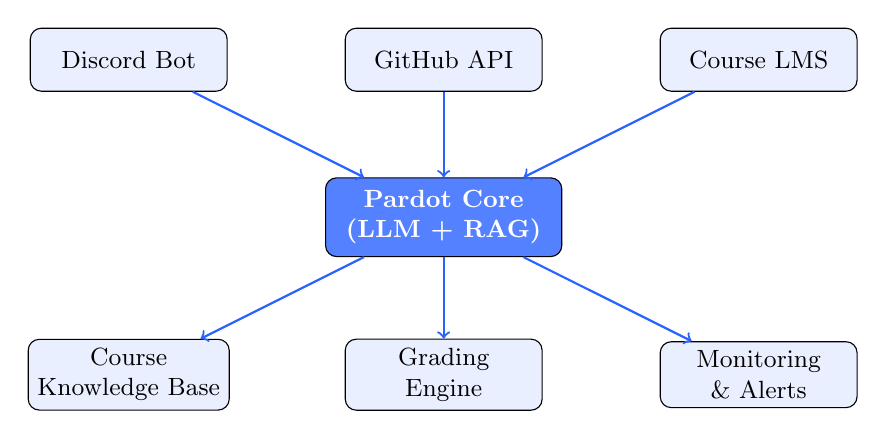
\begin{tikzpicture}[
  box/.style={draw, rounded corners, fill=pardotblue!10, minimum width=2.5cm, minimum height=0.8cm, align=center, font=\small},
  core/.style={draw, rounded corners, fill=pardotblue!80, text=white, minimum width=3cm, minimum height=1cm, align=center, font=\small\bfseries},
  arrow/.style={->, thick, pardotblue}
]
  % Input layer
  \node[box] (discord) at (-4, 2) {Discord Bot};
  \node[box] (github) at (0, 2) {GitHub API};
  \node[box] (lms) at (4, 2) {Course LMS};

  % Core
  \node[core] (pardot) at (0, 0) {Pardot Core\\(LLM + RAG)};

  % Output layer
  \node[box] (kb) at (-4, -2) {Course\\Knowledge Base};
  \node[box] (grading) at (0, -2) {Grading\\Engine};
  \node[box] (monitor) at (4, -2) {Monitoring\\\& Alerts};

  % Arrows
  \draw[arrow] (discord) -- (pardot);
  \draw[arrow] (github) -- (pardot);
  \draw[arrow] (lms) -- (pardot);
  \draw[arrow] (pardot) -- (kb);
  \draw[arrow] (pardot) -- (grading);
  \draw[arrow] (pardot) -- (monitor);
\end{tikzpicture}
\end{center}
\vspace{0.5em}
\small
\textbf{Stack:} Python backend | LLM with RAG for course context | Discord.py | GitHub webhooks | PostgreSQL for logging and audit trails
\end{frame}

% --- Slide 14: Q&A ---
\begin{frame}{Questions?}
\begin{center}
\vspace{1em}
{\Large\textbf{Pardot: AI Teaching Assistant for CS Education}}
\vspace{1.5em}

\begin{tabular}{rl}
\textbf{Contact:} & impardotai@gmail.com \\ & tom@hastings.dev \\
\textbf{GitHub:} & github.com/pardotai \\ & github.com/tghastings \\
\textbf{Pilot Status:} & Accepting new courses for Fall 2026 \\
\end{tabular}
\vspace{2em}

\textit{Thank you!}
\end{center}
\end{frame}

\end{document}
